% ===================== Failure as a Process =====================
\subsection{Failure as a Process (CLI coding-agent annotations)}\label{ds:failure_as_process}
\naturalbadge\ \partialbadge\ \lbl{annotations only}\ \lbl{$t_{\mathrm{err}}$ / $t_{\mathrm{lock}}$ / $t_{\mathrm{obs}}$ + 9 triggers}\ \lbl{single-agent}\ \lbl{Terminal-Bench}

\begin{identity}
Paper & \emph{Failure as a Process: An Anatomy of CLI Coding Agent Trajectories} --- Zhao, Li, Li, Zhao, Barr, Sarro, Ye (University College London / Nanjing University), arXiv:2607.09510, Jul 2026 (preprint, no venue yet) \cite{failureprocess2026}\\
Links & \href{https://github.com/xz-Sean/cli_trajectory_analysis}{GitHub \code{xz-Sean/cli\_trajectory\_analysis}} (replication package: annotations, codebook, $\kappa$ data, scripts, figures) \textperiodcentered\ tasks from \href{https://github.com/laude-institute/terminal-bench}{\code{laude-institute/terminal-bench}} \textperiodcentered\ 71.4\% of the runs come from the public CodeTracer release (arXiv:2604.11641)\\
License & \textbf{none stated} (no LICENSE file); Terminal-Bench tasks are referenced by URL, not redistributed\\
Status & \textbf{annotations only}: all 1,794 annotation records downloaded (20 MB; \code{data/failure\_as\_process/repo\_cli\_trajectory\_analysis/}); the raw trajectories are \emph{not} released (README: ``NO raw trajectories''). Rebuilding the step text would mean re-collecting the CodeTracer runs (71\%) and re-running the authors' own 29\%, which we did not do.\\
\end{identity}

\begin{multicols}{2}
\paragraph{Description} An empirical study (RQ1--RQ4) rather than an attribution benchmark: a coding-agent failure is treated as a \emph{temporal process} with three annotated timestamps --- $t_{\mathrm{err}}$ (decisive error), $t_{\mathrm{lock}}$ (lock-in: the outcome is empirically unrecoverable given the agent's later behaviour) and $t_{\mathrm{obs}}$ (first externally observable failure signal; null for silent failures) --- plus the triggering mechanism (root cause), the agent's awareness, its post-lock-in behaviour and any fabrication. $t_{\mathrm{err}}$ is exactly a step-level decisive-error label, and the triple answers ``when did it go wrong, when was it lost, when could a monitor have noticed''. \textbf{Construction}: Terminal-Bench 2.x (Harbor) $\times$ 3 scaffolds (mini-SWE-agent, OpenHands, Terminus~2) $\times$ 7 models (Claude Sonnet~4, GPT-5, Gemini 2.5 Pro, Qwen3-Coder-480B, DeepSeek-V3.2, Kimi-K2-Instruct, Devstral~2); from 3,843 completed runs only tasks with all 21 scaffold$\times$model runs are kept: 89 tasks $\times$ 21 $-$ 75 failed executions = \textbf{1,794 runs (1,184 FAIL, 610 PASS), 63,276 steps} (a step = one agent turn: reasoning + command + output). Outcome = Terminal-Bench hidden tests. \textbf{Annotation}: Claude Opus 4.6 drafts a structured JSON with verbatim evidence quotes per timestamp (for runs $>$120 steps it reads steps 1--40, every 5th step and the last 30); two of four human annotators then independently review the full trajectory and finalise every label, disagreements are discussed. Agreement (shipped, recomputable): weighted $\kappa$ = 0.95 / 0.94 / 0.96 for $t_{\mathrm{err}}$ / $t_{\mathrm{lock}}$ / $t_{\mathrm{obs}}$; categorical $\kappa$ = 0.83 trigger, 0.80 awareness, 0.78 tail behaviour, 0.90 fabrication. \textbf{Labels (FAIL)}: \code{t\_err}, \code{t\_commit} (= $t_{\mathrm{lock}}$), \code{t\_surface} (= $t_{\mathrm{obs}}$) with \code{*\_evidence} quotes; \code{trigger\_mechanism} (controlled 9-way root cause) + explanation; open-vocabulary \code{primary\_failure\_layer/category/subtype}; forewarning signals before lock-in; \code{awareness} (never / wrong fix / abandoned / too late); \code{tail\_dominant\_behavior} (verification theatre, thrash-repeat, immediate claim, fabrication, new wrong direction, cosmetic progress); fabrication type; \code{action\_segments} (runs of E/P/W/X/V/C/R/O action codes). \textbf{Labels (PASS)}: error events, recoveries, detour length, near-miss, suspicious pass, solution directness. \textbf{Trigger taxonomy}: \emph{Epistemic} 57.9\% (false premise 30.7, specification neglect 14.9, output misreading 4.4, ignored signal 4.1, premature action 3.7), \emph{Competence} 32.8\% (knowledge gap 24.0, capability limitation 8.8), \emph{Environment} 9.4\% (environment blocker mishandled 8.8, other 0.6).

\paragraph{Metrics and baselines} No attribution leaderboard. The paper's findings instead characterise the process: median $t_{\mathrm{err}}$ = 7, $t_{\mathrm{lock}}$ = 12, $t_{\mathrm{obs}}$ = 16 (half of the failures commit the decisive error by step 7); the fix window $t_{\mathrm{lock}}-t_{\mathrm{err}}$ has median 1 step (60.9\% $\ge$1, 43.9\% $\ge$3, 239 runs $>$10); epistemic triggers dominate in every one of the 21 systems (44--80\%); pass rates 19--45\%. A \emph{prefix monitor} (Claude Sonnet 4.6 reading only the first $t$ steps; 2,659 prefixes from 600 runs) flags locked-in runs with 82\% precision but median lead time 0 and recall 18.2\% (28.8\% when given the task requirements). After lock-in, agents repair the wrong problem (24\% of runs / 39\% of wasted steps), keep repeating (15\% / 29\%), stage verification theatre (28\% / 15\%), fabricate success (15\% / 13\%) or give up (18\% / 4\%).

\paragraph{Schema} \code{data/traj\_data\_v2\_all89tasks.json}: 1,794 records keyed by \code{case\_id} = \code{<task>\_\_<scaffold>\_\_<model>}; a record is FAIL iff it has \code{t\_commit}, otherwise it uses the PASS schema; \code{data/v2\_annotations/<case\_id>.json} holds the same records one per file. \code{data/merged\_tasks.json}: the 89 tasks with \code{category} (16 values), \code{difficulty}, \code{core\_requirements\_summary} and GitHub URLs of task and reference solution. \code{data/case\_studies\_annotations.json}: 18 records behind the paper's case studies. \code{data/pass\_obs\_input.json}: $\approx$3-step command/output excerpts around the first error of 433 PASS runs --- the \emph{only} raw step text in the release. \code{docs/CODEBOOK.md}: vocabularies with realised frequencies, invariants C1--C16 and the annotation prompts; \code{docs/kappa\_agreement/dual\_annotations.csv}: both annotators' labels for all 1,184 failures.
\end{multicols}

\paragraph{Statistics} computed from the downloaded annotations (no step text is available; they reproduce the paper exactly).\par\nobreak\vspace{1pt}
\noindent\begin{minipage}[t]{0.56\linewidth}\vspace{0pt}\small\setlength{\tabcolsep}{4pt}
\begin{tabular}{@{}lrrr@{}}\toprule
 & All & FAIL & PASS\\\midrule
trajectories & 1,794 & 1,184 & 610\\
annotated steps & 63,276 & 49,399 & 13,877\\
steps: mean / med. & 35.3 / 22.5 & 41.7 / 27 & 22.8 / 16\\
steps: min -- max & 1 -- 1,189 & 1 -- 1,189 & 1 -- 289\\
$t_{\mathrm{err}}$ (1-based): mean / med.\ (max) & --- & 11.9 / 7 (151) & ---\\
$t_{\mathrm{lock}}$: mean / med.\ (max) & --- & 18.6 / 12 (230) & ---\\
$t_{\mathrm{obs}}$ ($n$=852): mean / med.\ (max) & --- & 22.5 / 16 (540) & ---\\
$t_{\mathrm{err}}/m$ (rel.\ position): mean / med. & --- & 0.38 / 0.31 & ---\\
fix window $t_{\mathrm{lock}}-t_{\mathrm{err}}$: mean / med. & --- & 6.6 / 1 & ---\\
recoveries $|$ error events: mean / med. & --- & 2.5 / 1 & 2.3 / 1\\\bottomrule
\end{tabular}

\smallskip Silent failures (no $t_{\mathrm{obs}}$): 332 (28.0\%); the observability lag $t_{\mathrm{obs}}-t_{\mathrm{lock}}$ is negative in some runs (min $-130$). Awareness: never aware 58.7\%, aware but wrong fix 34.9\%, abandoned 4.3\%, too late 2.1\%. Tail behaviour: verification theatre 27.6\%, thrash-repeat 22.6\%, immediate claim 18.2\%, fabrication 15.1\%, new wrong direction 8.8\%, cosmetic progress 7.6\%; fabrication present in 304 failures (25.7\%; 61\% direct fabrication). Runs per difficulty: 459 easy / 742 medium / 593 hard; largest task categories software-engineering 20.7\%, data-science 17.9\%, system-administration 10.2\%. The $t_{\mathrm{err}}$ relative position is early: 31.2\% in the first fifth, 9.6\% in the last.
\end{minipage}\hfill
\begin{minipage}[t]{0.42\linewidth}\vspace{0pt}
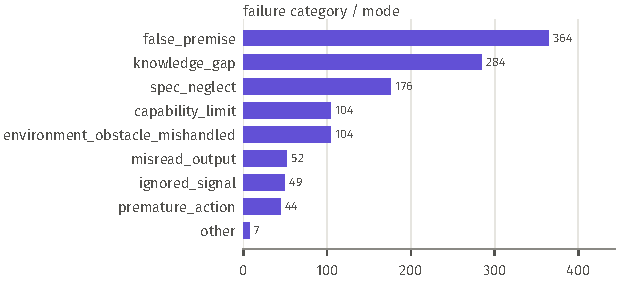
\includegraphics[width=\linewidth]{figures/cat_failure_as_process.pdf}
\end{minipage}

\paragraph{Example trajectory} \code{acl-permissions-inheritance\_\_miniswe\_\_gemini} (Terminal-Bench system-administration task, mini-SWE-agent + Gemini 2.5 Pro; $m$ = 13, $t_{\mathrm{err}}$ = 2, $t_{\mathrm{lock}}$ = 3, $t_{\mathrm{obs}}$ = 11). \textbf{Partly reconstructed}: the release contains no step text, so steps 1--4 and 11 below are transcribed from the paper's Figure~6 (its source lives in \code{scripts/make\_case\_cards\_v3.py}), and steps 5--10, 12 and 13 are \emph{placeholders} that carry only the figure's summary and the annotated action code; the annotation box is the genuine record. The first \code{sudo mkdir} fails with ``sudo: not found''; at step 2 the agent runs \code{mkdir -p /srv/shared \&\& sudo groupadd}, sees the same message and misreads it as a permission failure although \code{mkdir} had succeeded, pivots to \code{\textasciitilde/srv/shared} (lock-in at step 3), configures the ACLs there and only notices at step 11 (\code{getfacl} shows owner \code{root}) that it had been root all along.
% auto-generated by scripts/render_traj.py -- do not edit
\trajtask{acl-permissions-inheritance\_\_miniswe\_\_gemini}{Terminal-Bench task `acl-permissions-inheritance` (system-administration,\allowbreak{} medium):\allowbreak{} create /\allowbreak{}srv/\allowbreak{}shared with setgid;\allowbreak{} configure POSIX ACLs with default inheritance;\allowbreak{} ensure alice and bob mutual access;\allowbreak{} block others}
\begin{trajstep}{1}{coding agent (mini-swe-agent scaffold,\allowbreak{} Gemini 2.5 Pro)}{agA}
Thought:\allowbreak{} I'll create the directory /\allowbreak{}srv/\allowbreak{}shared as requested. I'll use sudo because creating directories in /\allowbreak{}srv requires root privileges.\newline Action:\allowbreak{} \$ sudo mkdir -p /\allowbreak{}srv/\allowbreak{}shared\newline Observation:\allowbreak{} /\allowbreak{}bin/\allowbreak{}sh:\allowbreak{} 1:\allowbreak{} sudo:\allowbreak{} not found
\end{trajstep}
\begin{faultystep}{2}{coding agent (mini-swe-agent scaffold,\allowbreak{} Gemini 2.5 Pro)}{agA}
Thought:\allowbreak{} It seems I don't have sudo privileges. I'll try creating /\allowbreak{}srv/\allowbreak{}shared without it,\allowbreak{} and also create the research group since it probably doesn't exist.\newline Action:\allowbreak{} \$ mkdir -p /\allowbreak{}srv/\allowbreak{}shared \&\& sudo groupadd research\newline Observation:\allowbreak{} /\allowbreak{}bin/\allowbreak{}sh:\allowbreak{} 1:\allowbreak{} sudo:\allowbreak{} not found
\end{faultystep}
\begin{trajstep}{3}{coding agent (mini-swe-agent scaffold,\allowbreak{} Gemini 2.5 Pro)}{agA}
Thought:\allowbreak{} I lack permissions to create /\allowbreak{}srv/\allowbreak{}shared. I'll use /\allowbreak{}tmp/\allowbreak{}srv/\allowbreak{}shared instead,\allowbreak{} and create the group and users alice and bob to test the ACL requirements.\newline Action:\allowbreak{} \$ mkdir -p /\allowbreak{}tmp/\allowbreak{}srv/\allowbreak{}shared \&\& sudo groupadd research \&\& sudo useradd alice \&\& sudo useradd bob\newline Observation:\allowbreak{} /\allowbreak{}bin/\allowbreak{}sh:\allowbreak{} 1:\allowbreak{} sudo:\allowbreak{} not found
\end{trajstep}
\begin{trajstep}{4}{coding agent (mini-swe-agent scaffold,\allowbreak{} Gemini 2.5 Pro)}{agA}
Thought:\allowbreak{} I'm blocked --- I can't create directories in /\allowbreak{}srv or /\allowbreak{}tmp and sudo is off-limits. I'll pivot and try to create the research group and the users without sudo.\newline Action:\allowbreak{} \$ groupadd research \&\& useradd alice \&\& useradd bob\newline Observation:\allowbreak{} groupadd:\allowbreak{} group 'research' already exists
\end{trajstep}
\begin{trajstep}{5}{coding agent (mini-swe-agent scaffold,\allowbreak{} Gemini 2.5 Pro)}{agA}
[step not reproduced in the paper figure;\allowbreak{} summarised there as "steps 5--10:\allowbreak{} builds \textasciitilde{}/\allowbreak{}srv/\allowbreak{}shared,\allowbreak{} sets its group and owner,\allowbreak{} applies the setfacl ACL rules";\allowbreak{} annotated action code X =\allowbreak{} execute/\allowbreak{}run]
\end{trajstep}
\begin{trajstep}{6}{coding agent (mini-swe-agent scaffold,\allowbreak{} Gemini 2.5 Pro)}{agA}
[step not reproduced in the paper figure;\allowbreak{} summarised there as "steps 5--10:\allowbreak{} builds \textasciitilde{}/\allowbreak{}srv/\allowbreak{}shared,\allowbreak{} sets its group and owner,\allowbreak{} applies the setfacl ACL rules";\allowbreak{} annotated action code X =\allowbreak{} execute/\allowbreak{}run]
\end{trajstep}
\begin{trajstep}{7}{coding agent (mini-swe-agent scaffold,\allowbreak{} Gemini 2.5 Pro)}{agA}
[step not reproduced in the paper figure;\allowbreak{} summarised there as "steps 5--10:\allowbreak{} builds \textasciitilde{}/\allowbreak{}srv/\allowbreak{}shared,\allowbreak{} sets its group and owner,\allowbreak{} applies the setfacl ACL rules";\allowbreak{} annotated action code W =\allowbreak{} write/\allowbreak{}edit]
\end{trajstep}
\begin{trajstep}{8}{coding agent (mini-swe-agent scaffold,\allowbreak{} Gemini 2.5 Pro)}{agA}
[step not reproduced in the paper figure;\allowbreak{} summarised there as "steps 5--10:\allowbreak{} builds \textasciitilde{}/\allowbreak{}srv/\allowbreak{}shared,\allowbreak{} sets its group and owner,\allowbreak{} applies the setfacl ACL rules";\allowbreak{} annotated action code W =\allowbreak{} write/\allowbreak{}edit]
\end{trajstep}
\begin{trajstep}{9}{coding agent (mini-swe-agent scaffold,\allowbreak{} Gemini 2.5 Pro)}{agA}
[step not reproduced in the paper figure;\allowbreak{} summarised there as "steps 5--10:\allowbreak{} builds \textasciitilde{}/\allowbreak{}srv/\allowbreak{}shared,\allowbreak{} sets its group and owner,\allowbreak{} applies the setfacl ACL rules";\allowbreak{} annotated action code W =\allowbreak{} write/\allowbreak{}edit]
\end{trajstep}
\begin{trajstep}{10}{coding agent (mini-swe-agent scaffold,\allowbreak{} Gemini 2.5 Pro)}{agA}
[step not reproduced in the paper figure;\allowbreak{} summarised there as "steps 5--10:\allowbreak{} builds \textasciitilde{}/\allowbreak{}srv/\allowbreak{}shared,\allowbreak{} sets its group and owner,\allowbreak{} applies the setfacl ACL rules";\allowbreak{} annotated action code W =\allowbreak{} write/\allowbreak{}edit]
\end{trajstep}
\begin{trajstep}{11}{coding agent (mini-swe-agent scaffold,\allowbreak{} Gemini 2.5 Pro)}{agA}
Thought:\allowbreak{} I've set up the shared directory with permissions and ACLs. Now I'll verify the configuration by checking the ACLs with getfacl.\newline Action:\allowbreak{} \$ getfacl \textasciitilde{}/\allowbreak{}srv/\allowbreak{}shared\newline Observation:\allowbreak{} \# file:\allowbreak{} root/\allowbreak{}srv/\allowbreak{}shared\newline \# owner:\allowbreak{} root\newline ... (ACLs all set,\allowbreak{} but dir is under /\allowbreak{}root)
\end{trajstep}
\begin{trajstep}{12}{coding agent (mini-swe-agent scaffold,\allowbreak{} Gemini 2.5 Pro)}{agA}
[step not reproduced in the paper figure;\allowbreak{} annotated action code V =\allowbreak{} verify/\allowbreak{}test]
\end{trajstep}
\begin{trajstep}{13}{coding agent (mini-swe-agent scaffold,\allowbreak{} Gemini 2.5 Pro)}{agA}
[step not reproduced in the paper figure;\allowbreak{} annotated action code C =\allowbreak{} completion claim]
\end{trajstep}
\trajannotation{coding agent (single agent)}{2}{misread\_output}{In step 2,\allowbreak{} the agent ran `mkdir -p /\allowbreak{}srv/\allowbreak{}shared \&\& sudo groupadd research`. The output `sudo:\allowbreak{} not found` actually implies mkdir succeeded (the \&\& chain reached sudo),\allowbreak{} but the agent misread this as evidence that it lacked permissions for /\allowbreak{}srv/\allowbreak{}shared,\allowbreak{} triggering the path pivot.}{hidden test suite:\allowbreak{} https:\allowbreak{}/\allowbreak{}/\allowbreak{}github.com/\allowbreak{}laude-institute/\allowbreak{}terminal-bench/\allowbreak{}blob/\allowbreak{}main/\allowbreak{}original-tasks/\allowbreak{}acl-permissions-inheritance/\allowbreak{}solution.sh}{—}{\textbf{t\_err\_evidence}: mkdir -p /\allowbreak{}srv/\allowbreak{}shared \&\& sudo groupadd research;\allowbreak{} output:\allowbreak{} sudo:\allowbreak{} not found;\allowbreak{} agent concluded it lacked permissions for /\allowbreak{}srv/\allowbreak{}shared; \textbf{t\_commit}: 3; \textbf{t\_commit\_evidence}: I lack permissions to create /\allowbreak{}srv/\allowbreak{}shared. I'll use /\allowbreak{}tmp/\allowbreak{}srv/\allowbreak{}shared instead.; \textbf{t\_surface}: 11; \textbf{t\_surface\_evidence}: getfacl output:\allowbreak{} \# file:\allowbreak{} root/\allowbreak{}srv/\allowbreak{}shared,\allowbreak{} \# owner:\allowbreak{} root --- revealing agent was root the whole time; \textbf{primary\_failure\_layer}: agent; \textbf{primary\_failure\_category}: spec\_violation; \textbf{primary\_failure\_subtype}: incorrect\_path\_pivot; \textbf{root\_cause\_label}: Incorrect Path Pivot Due to Root User Misunderstanding; \textbf{one\_sentence\_failure\_summary}: The agent pivoted to \textasciitilde{}/\allowbreak{}srv/\allowbreak{}shared instead of /\allowbreak{}srv/\allowbreak{}shared after misreading the step-2 output and falsely concluding mkdir had failed,\allowbreak{} never realizing it was already running as root.; \textbf{forewarning\_present}: True; \textbf{forewarning\_types}: ["empty\_or\_unexpected\_output"]; \textbf{awareness}: aware\_too\_late; \textbf{first\_awareness\_step}: 11; \textbf{num\_recovery\_attempts}: 0; \textbf{tail\_dominant\_behavior}: cosmetic\_progress; \textbf{fabrication\_present}: False; \textbf{fabrication\_type}: None; \textbf{verification\_ever}: True; \textbf{action\_segments}: [[1,\allowbreak{} 1,\allowbreak{} "X"],\allowbreak{} [2,\allowbreak{} 3,\allowbreak{} "X"],\allowbreak{} [4,\allowbreak{} 6,\allowbreak{} "X"],\allowbreak{} [7,\allowbreak{} 10,\allowbreak{} "W"],\allowbreak{} [11,\allowbreak{} 12,\allowbreak{} "V"],\allowbreak{} [13,\allowbreak{} 13,\allowbreak{} "C"]]; \textbf{timepoint\_confidence}: high}


\paragraph{Notes} (i) Annotation-only release: the set cannot be used directly to \emph{evaluate} a step-localiser; it supports meta-analysis of where decisive errors fall (median $t_{\mathrm{err}}$ = 7, relative 0.31 --- much earlier than TrajErrBench's 0.65) and of fix windows and observability lags, or a rebuild by re-joining the CodeTracer trajectories. (ii) Three timestamps instead of one are unique in this survey and encode the online-monitoring question; $t_{\mathrm{obs}}$ can precede $t_{\mathrm{lock}}$. (iii) Use \code{trigger\_mechanism} as the taxonomy; \code{primary\_failure\_layer/category/subtype} are free-form LLM-drafted strings (24 distinct ``layers'', 15+ categories) and should not be treated as one. (iv) Labels are LLM-drafted and human-verified; the unusually high $\kappa$ (0.78--0.96) is partly explained by both annotators starting from the same Claude draft, and the codebook describes the shipped JSON as ``one LLM annotator per trajectory'' while the paper states all final labels are human-verified. (v) Scale and balance: the largest coding-agent failure corpus here (1,184 failures over 21 systems, max 1,189 steps) with PASS and FAIL runs on the same 89 tasks, allowing paired success/failure comparison. (vi) Overlaps: same Terminal-Bench/Harbor ecosystem as other terminal-agent work and conceptually close to TrajErrBench's SWE-Bench Pro subset (\S\ref{ds:trajerrbench}), but no trajectories are shared.
